\documentclass[11pt]{article}
\renewcommand{\baselinestretch}{1.20} 
\usepackage[utf8]{inputenc}
\usepackage[danish]{babel}
\usepackage{graphicx}
\usepackage{wrapfig}
\usepackage{subcaption}
\usepackage{geometry}
 \geometry{
 a4paper,
 total={170mm,237mm},
 left=20mm,
 top=30mm,
 }
 
\setlength{\abovecaptionskip}{15pt plus 3pt minus 2pt}

\rhead{Social hidden Messages 2018}
\lhead{Gruppe: B-125}
\chead{P2 - Rapport}
\rfoot{Page \thepage}

\title{Positioning Tables and Figures}
\author{ }
\date{ }

\begin{document}

\section{Titel}

\begin{figure}[h]
    \begin{subfigure}[t]{0.5\textwidth}
        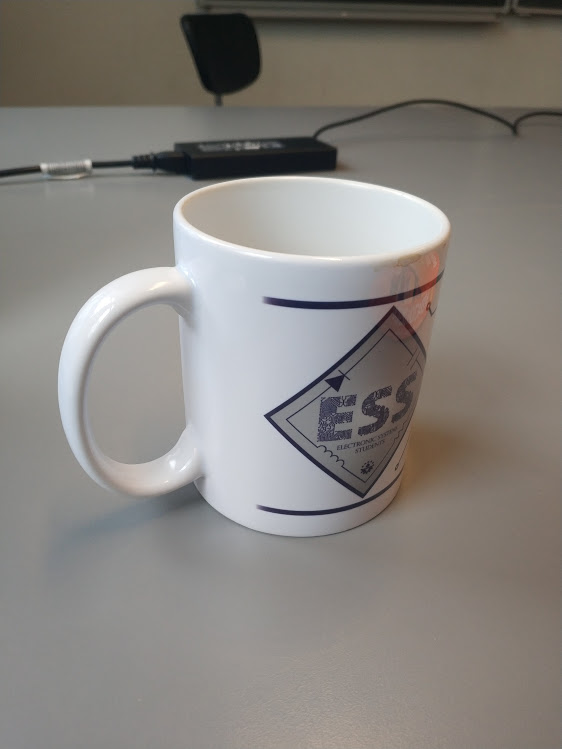
\includegraphics[scale=0.4]{InteraktionsDesign/Assets/kop.jpg}
        \caption{The cup has a great usability in that its easy to learn how to use it properly. The tap on the cup stands out from the otherwise cylinder shaped cup, which makes it very recognisable. The tap the cup has multiple purposes usability-wise, for instance it makes it safer to use when the cup contains hot liquid. The tap also makes for added efficiency and overall convenience.
        Moreover, the tap is shaped in such a way that it accommodates several fingers allowing for a solid grip with a range of hand sizes. The smooth finish of the handle is used for a pleasant user experience. The sense of control over the cup also adds to this pleasantness of the experience}
        \label{fig:cup}
    \end{subfigure}
    \begin{subfigure}[t]{0.5\textwidth}
        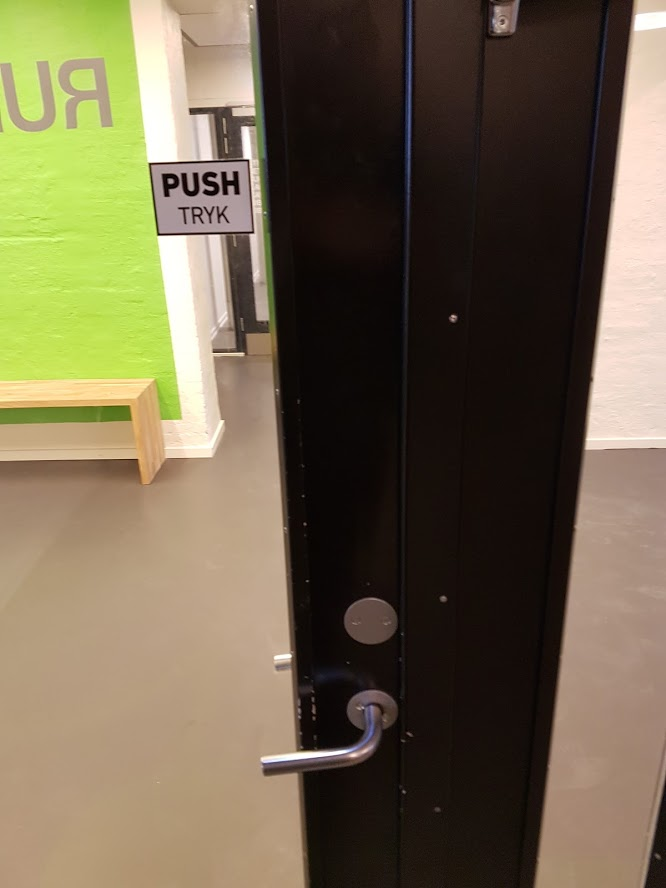
\includegraphics[scale=0.4]{InteraktionsDesign/Assets/door.jpg}
        \caption{The cup has a great usability in that its easy to learn how to use it properly. The tap on the cup stands out from the otherwise cylinder shaped cup, which makes it very recognisable. The tap the cup has multiple purposes usability-wise, for instance it makes it safer to use when the cup contains hot liquid. The tap also makes for added efficiency and overall convenience.}
        \label{fig:cup}
    \end{subfigure}
\end{figure}


\end{document}